\documentclass[8pt,a4paper]{extarticle}

\usepackage[margin=0.8cm, landscape]{geometry}
\usepackage[utf8]{inputenc}
\usepackage{CJKutf8}
\usepackage{multicol}
\usepackage{amsmath, amssymb}
\usepackage{graphicx}
\usepackage{xcolor}
\usepackage{enumitem}
\usepackage{titlesec}
\usepackage{caption}
\usepackage{float}

\definecolor{sectionbg}{RGB}{230, 230, 230}
\setlist{nosep, leftmargin=1.2em}
\setlength{\columnsep}{0.4cm}

\setlength{\parindent}{0pt}

\titleformat{\section}
  {\normalfont\large\bfseries}{\thesection}{1em}{}[{\titlerule[0.8pt]}]
\titlespacing*{\section}{0pt}{2pt}{2pt}
\titlespacing*{\subsection}{0pt}{0.4\baselineskip}{0.1\baselineskip}

\newcommand{\entry}[1]{\vspace{3pt}\noindent\textbf{#1：}}

\captionsetup{skip=1pt,belowskip=0pt,aboveskip=0pt}

\begin{document}
\begin{CJK*}{UTF8}{gbsn}

\noindent \small \textbf{Intro2CV Cheatsheet} by \underline{Kristina} \hfill \today

\begin{multicols*}{4}

\section{3D Vision}

\subsection*{Camera Model}

\entry{Pinhole Camera}$x' = f\frac{x}{z},\ y' = f\frac{y}{z}$ (focal length $f$)

aperture big - blur; aperture small - dark

\entry{Camera and Lense}$z' = f + z_0,\ f = \frac{R}{2(n-1)}$

specific "in focus" distance - depth of field

camera parameters: intrinsics \& extrinsics

$k,l$: pixel/m $\alpha = f \cdot k,\ \beta = f \cdot l$

convert between Euclidian \& Homogeneous coordinates

$P' = \left[\begin{array}{cc}
     \alpha x + c_x z  \\
     \beta y + c_y z \\
     z
\end{array} \right] = \left[ \begin{matrix}
    \alpha & -\alpha \cot\theta & c_x & 0 \\
     0 & \beta/\sin\theta & c_y & 0 \\
     0 & 0 & 1 & 0 
\end{matrix}\right] \left[\begin{array}{cc}
    x \\ y  \\ z \\ 1
\end{array}\right] = M P = K [I \ 0] P = K[I \ 0]\left[\begin{matrix}
     R& T\\
     0& 1
\end{matrix}\right]_{4*4} P_w = K [R \ T] P_w$

$R = R_x(\alpha) R_y(\beta) R_z(\gamma)$, usually $\theta = \pi/2$

$M = [m_1, m_2, m_3]^T, (\frac{m_1P_W}{m_2P_w}, \frac{m_2P_w}{m_3P_w})$ in E

\subsection*{Depth Images}

\entry{Depth Image}a 2.5D representation

can't recover $(x,y,z)$ or point-to-point dist without $K$

backprojection: given $K$, $(u,v) = (\alpha\frac{x}{z}+c_x, \beta\frac{y}{z}+c_y)$

Stereo sensors: $u-u' = \frac{B\cdot f}{z} = $disparity

Active stereo: replace one camera with a projector

\entry{Voxel Grid}regular occupancy grid in 3D, easy to index and run 3D conv, but memory/compute is $O(n^3)$

+: regular structure, compatible with conv nets

-: surface location is coarse, upsampling is hard, voxelization loses detail

\subsection*{Mesh}

graph \{vertex, edge\}

\entry{Triangle Mesh}$V=\{v_i\}\subset \mathbb{R}^3,\ E\subset V\times V,\ F\subset V\times V\times V$

stores explicit surface + topology; more compact than dense voxel grid, but irregular and harder for CNN-like processing

\subsection*{Point Cloud}

point cloud = surface + sampling

\entry{Uniform sampling}triangle $v_1, v_2, v_3$

$x = v_3 + a_1(v_1-v_3)+ a_2(v_2-v_3)$, $a_1, a_2 \in [0,1]$

+: easiest; -: irregularly spaced sampling

\entry{Farthest Point Sampling (FPS)}NP-hard, greedy

iteratively select

\entry{Distance metrics}

Chamfer: $\displaystyle\sum_{x \in S_1}\displaystyle\min_{y \in S_2}||x-y||_2 + \displaystyle\sum_{y \in S_2}\displaystyle\min_{x \in S_1}||x-y||_2$

Earth Mover's: $\displaystyle\min_{\phi: S_1 \to S_2} \displaystyle\sum_{x \in S_1} ||x-\phi(x)||_2$

CD - insensitive to sampling; EMD - sensitive

\subsection*{Implicit Field}

\entry{Signed Distance Function}$F = $ dist 2 surface

\entry{2D Marching Square}extract zero iso-surface

thershold; binary; T/F; contour; linear interpolation

\entry{Implicit shape}represent shape by a func on space

$f(x)=0$:surface;$<0$:inside;$>0$:outside

other choices: unsigned distance / occupancy network

\entry{SDF}collision check; continuous geometry storage

query any 3D point (not storing only surface samples)

\entry{3D Marching Cube}3D version of marching square

ambiguity $\rightarrow$ holes; larger local context / better tables

\entry{Mesh $\leftrightarrow$ SDF}sample points around mesh, compute nearest-surface distance, assign sign

zero iso-surface can be converted back to mesh by marching cube

\subsection*{3D Deep Learning}

\entry{DeepSDF}learn continuous SDF with neural network

sample more points near the zero level set if final output uses marching cube

Eikonal equation: $||\nabla f(x)||_2 = 1$

single shape: overfit one network; multiple shapes: add latent code

\entry{NeRF}for novel view synthesis, map $(x,d)\rightarrow (\sigma,c)$

$\sigma$:density/attenuation $c$:emitted color $d$:viewing dir

ray $r(t)=o+td$, render by volume integration along the ray

$\alpha_i = 1-\exp(-\sigma_i\delta_i),\ T_i = \displaystyle\prod_{j<i}(1-\alpha_j),\ C = \displaystyle\sum_i T_i\alpha_i c_i$

\entry{3D Gaussian Splatting (3DGS)}parameterize scene by sparse anisotropic 3D Gaussians

projected 3D Gaussian becomes 2D Gaussian; same volume rendering idea, but explicit and fast

parameterize only where density is nonzero

\entry{PointNet}unordered $\rightarrow$ permutation invariant NN

shared MLP on each point + symmetric pooling (max)

robust to resolution/noise; weakness: no local context

\begin{figure}[H]
    \centering
    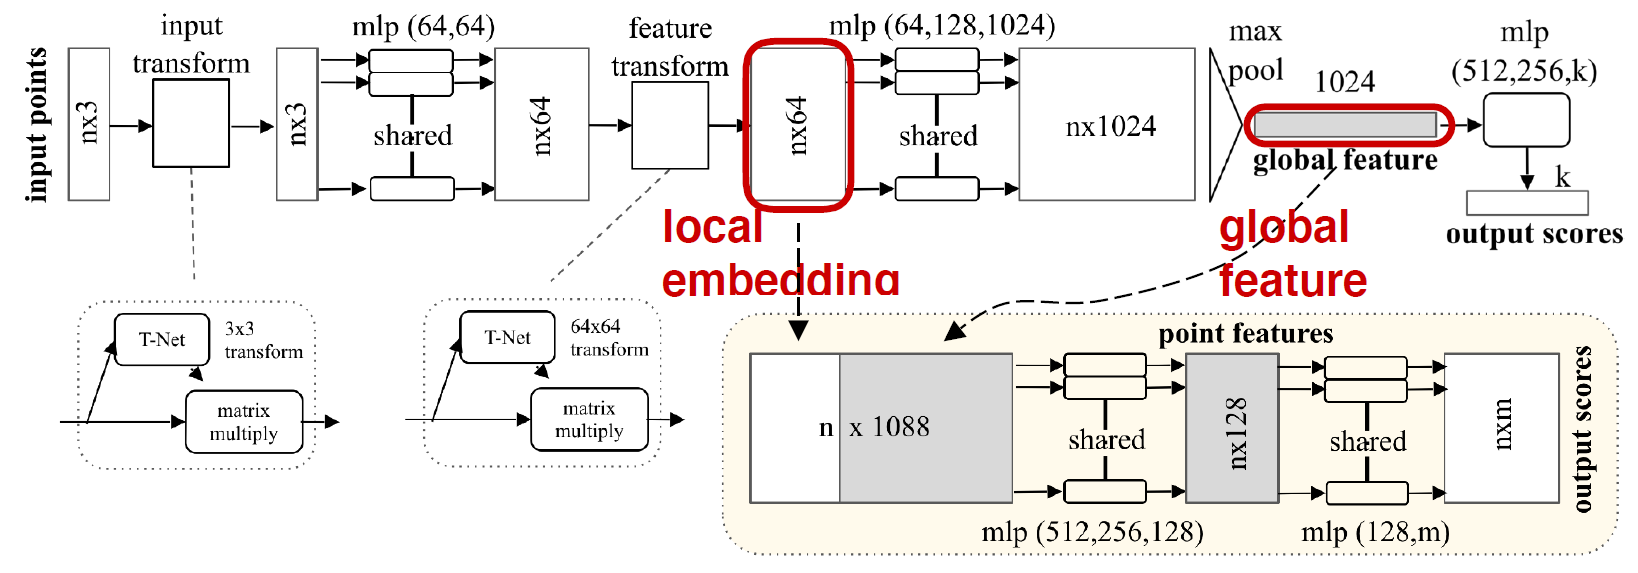
\includegraphics[width=\linewidth]{PointNet.png}
    \caption{PointNet Implementation}
\end{figure}

\entry{PointNet++}hierarchical local PointNet

sample centers by FPS, group neighbors, shared MLP in local region, then maxpool

downsample by grouping; upsample by interpolation + skip-link

similar to local conv, but all points in one neighborhood are treated isotropically

\entry{Ball Query}collect local neighborhood within radius

ball size and max queried points are hyperparameters

relative coordinates $x-x_c$ help extract translation-invariant local geometry feature

\entry{Set Abstraction}FPS + grouping + local PointNet

hierarchical feature learning with local translation invariance + permutation invariance

\entry{Segmentation in PointNet++}3D interpolation + unit PointNet + skip link concatenation

for new points, interpolate features from nearest neighbors with inverse-distance weights

\entry{Voxel Networks}3D CNN on volumetric data

easy extension of 2D conv, but dense 3D kernels are expensive and voxelization loses information

\entry{Sparse Conv}voxelize space, hash only active voxels

+: efficient on large scenes, similar inductive bias to 2D conv

-: quantization / discretization error, resolution limit

\begin{figure}[H]
    \centering
    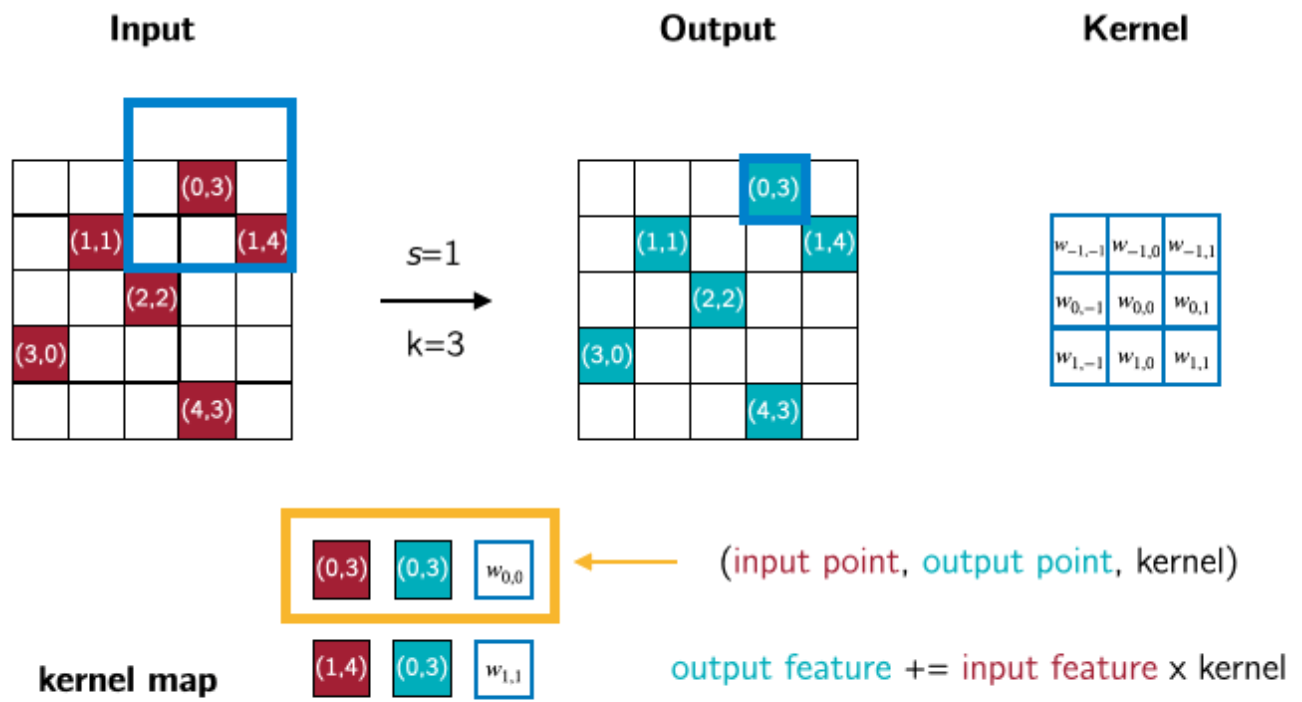
\includegraphics[width=\linewidth]{SparseConvolution.png}
    \caption{Sparse Convolution}
\end{figure}

\entry{Sparse Conv vs Point Cloud Nets}

sparse conv: spatially anisotropic kernels, efficient indexing, good for large scenes

point cloud nets: higher resolution, easier for quick use, but FPS / ball query can be slow

\section{Sequential Models}

\subsection*{RNN}

an internal state updated as the sequence is processed

$h_t = f_W(h_{t-1}, x_t),\ y_t = f_{W_{hy}}(h_t)$

recurrence formula - same func \& para each time step

\entry{Vanilla RNN}a single hidden vector $\mathbf{h}$

$h_t = \tanh(W_{hh}h_{t-1} + W_{xh}x_t),\ y_t = W_{hy}h_t$

gradient: $\frac{\partial L}{\partial W} = \displaystyle\sum_{t=1}^T \frac{\partial L_t}{\partial W},\ \frac{\partial L_t}{\partial W} = \frac{\partial L_T}{\partial h_t} \frac{\partial h_t}{\partial h_{t-1}} \cdots \frac{\partial h_0}{\partial W}$

\begin{figure}[H]
    \centering
    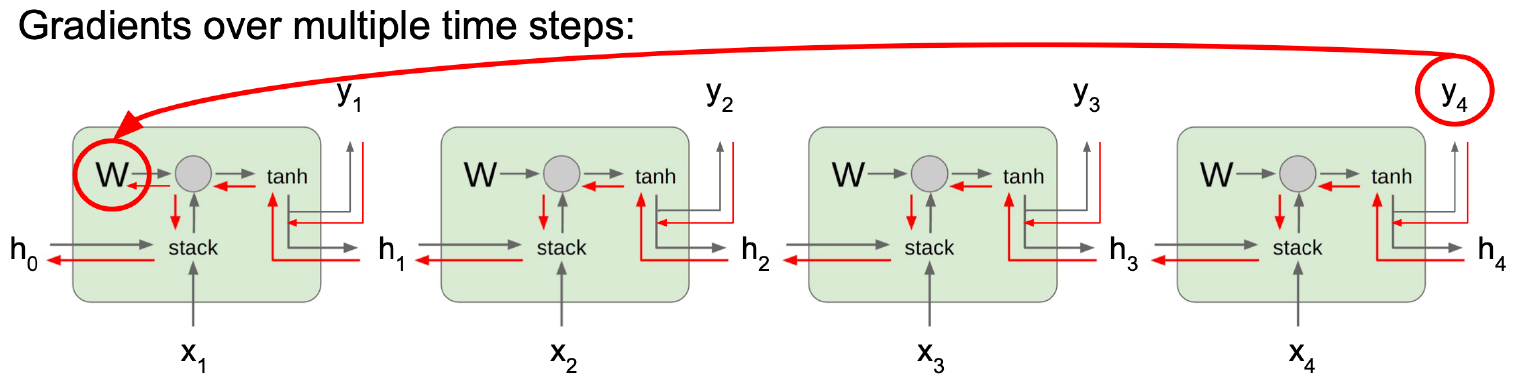
\includegraphics[width=\linewidth]{VanillaRNN.png}
    \caption{Vanilla RNN Gradient Flow}
\end{figure}

truncated backpropagation: run through chunks of seq

sequence length: $\Delta T$, only learn shorter relationship

input $\rightarrow$ (tokenizer) $\rightarrow$ embedding $\rightarrow$ hidden $\rightarrow$ output

\entry{Sampling}greedy(determine) / weighted(wrong)

Exhaustive Search: $P(y|x) = \displaystyle\prod_{t-1}^T P(y_t|y_1,\cdots,y_{t-1},x)$

Beam Search: keep $k$ most probable sequence (efficient)

$\frac{\partial h_t}{\partial h_{t-1}} = \tanh'(W_{hh}h_{t-1}+W_{xh}x_t)W_{hh}$

$\tanh'(W_{hh}h_{t-1}+W_{xh}x_t)$ always $<1$: vanish gradients

more dependent on long-term memory, not near effects

$W_{hh}$ largest singularity $>1$: explode; $<1$: vanish

exploding - gradient clipping (scale)

vanishing - change RNN architecture

\subsection*{Long-Short Term Memory (LSTM)}

$\left(\begin{array}{cc}
    i \\ f \\ o \\ g
\end{array}\right) = \left(\begin{array}{cc}
    \sigma \\ \sigma \\ \sigma \\ \tanh
\end{array}\right) W \left(\begin{array}{cc}
    h_{t-1} \\ x_t
\end{array}\right)$, 4 gates

$c_t = f \odot c_{t-1} + i \odot g,\ h_t = o \odot \tanh(c_t)$

Input-whether to write to cell; Forget-whether to erase

Output-how much to reveal; Gate-how much to write

only elementwise multiplication, no matrix mul by $W$

doesn't guarantee no exploding/vanishing

\entry{Gated Recurrent Unit (GRU)}: other variant

\subsection*{Image Caption Using RNN}

$b_v = W_{hi}[CNN_{\theta_c}(I)]$

$h_t = f(W_{ht}x_t + W_{hh}h_{t-1} + b_h + 1(t=1) \odot b_v)$

special token: $<$END$>$ (finish)

small dataset: nearest neighbor (text/caption retrieval)

\section{Attention \& Transformer}

\subsection*{Attention}

\entry{Sequence to Sequence}

Encoder: $h_t = f_W{x_t, h_{t-1}}$

Decoder: $s_t = g_U(y_{t-1}, s_{t-1})$

train: $y$ correct input; wrong output cross-entropy loss

test: $y_t$ input the output of $y_{t-1}$

problem: input sequence through fixed size $c$

alignment scores: $e_{t,i} = f_{att}(s_{t-1}, h_i)$ (linear layer)

attention weights: $\sum_i a_{t,i} =1$

context vector: $c_t = \sum_i a_{t,i}h_i$

all differentiable, no supervision on attention weights

Query vects \& Data vecs transformed into Output vecs

each query attend to all data vec and give 1 output vec

inputs: query vec - $\mathbf{q}[D_X]$ / data vec - $\mathbf{X}[N_X \times D_X]$

computation: similarities - $e[N_X] \ e_{i} = \mathbf{q} \cdot \mathbf{X_i} / \sqrt{D_X}$ (scaled) / attention weights - $a = softmax(e) [N_X]$ / output vec - $\mathbf{y} = \sum_i a_i\mathbf{X_i} [D_X]$

% \begin{figure}[H]
%     \centering
%     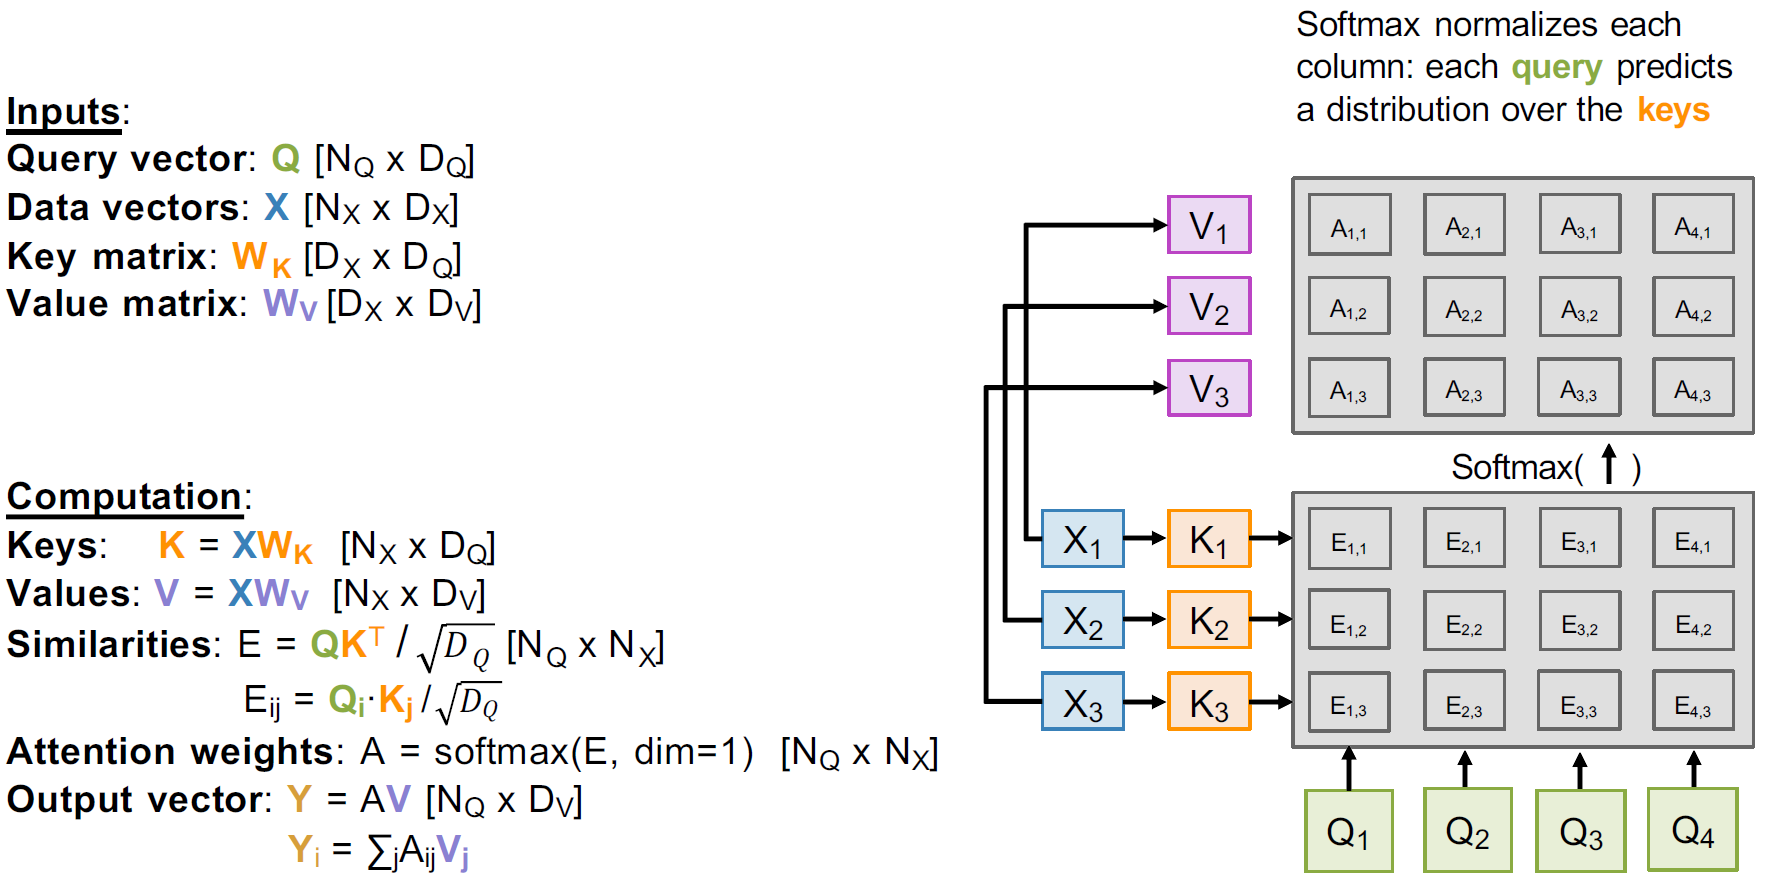
\includegraphics[width=\linewidth]{AttentionLayer.png}
%     \caption{Attention Layer}
% \end{figure}

% \begin{figure}[H]
%     \centering
%     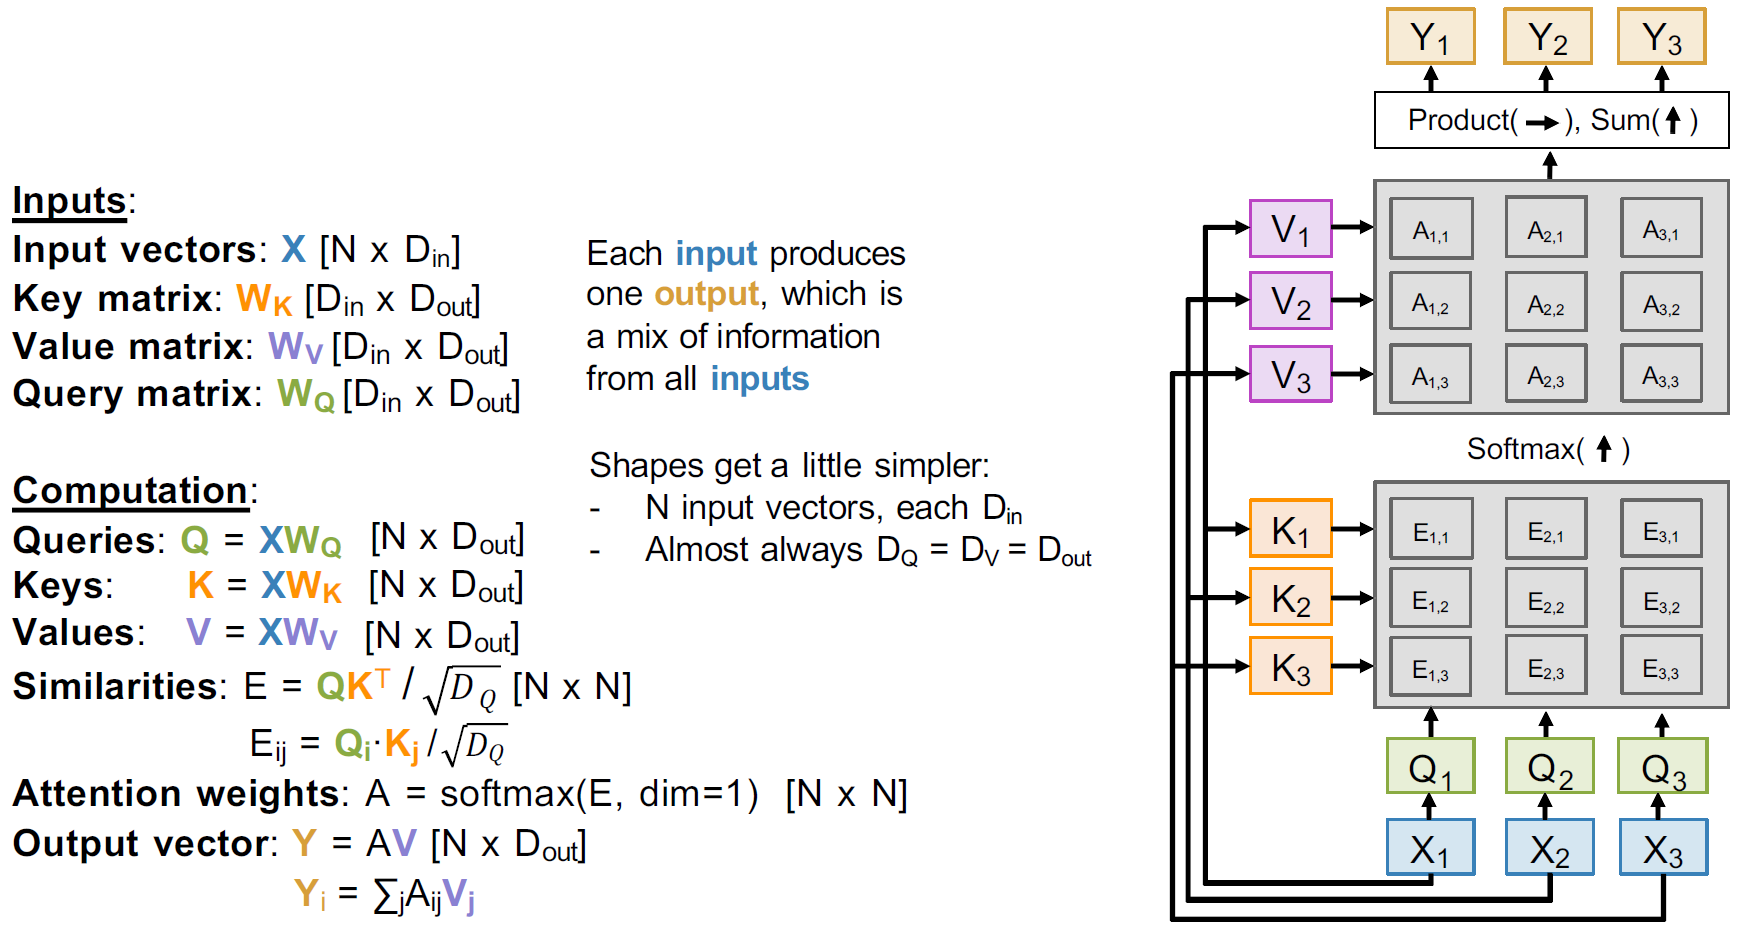
\includegraphics[width=\linewidth]{SelfAttentionLayer.png}
%     \caption{Self-Attention Layer}
% \end{figure}

permutation equivariant ($F(\sigma(X)) = \sigma(F(X))$)

\entry{Position embedding}a fixed vector of index

Rotary Positional Embedding: encode relative pos

$(R(\theta_i)q_i)^T (R(\phi_j)k_j) = q_i^T R(\phi_j-\theta_i) k_j$

Causal mask: prevent looking ahead while training

\entry{Multi-headed self attention}parallel H heads

\begin{figure}[H]
    \centering
    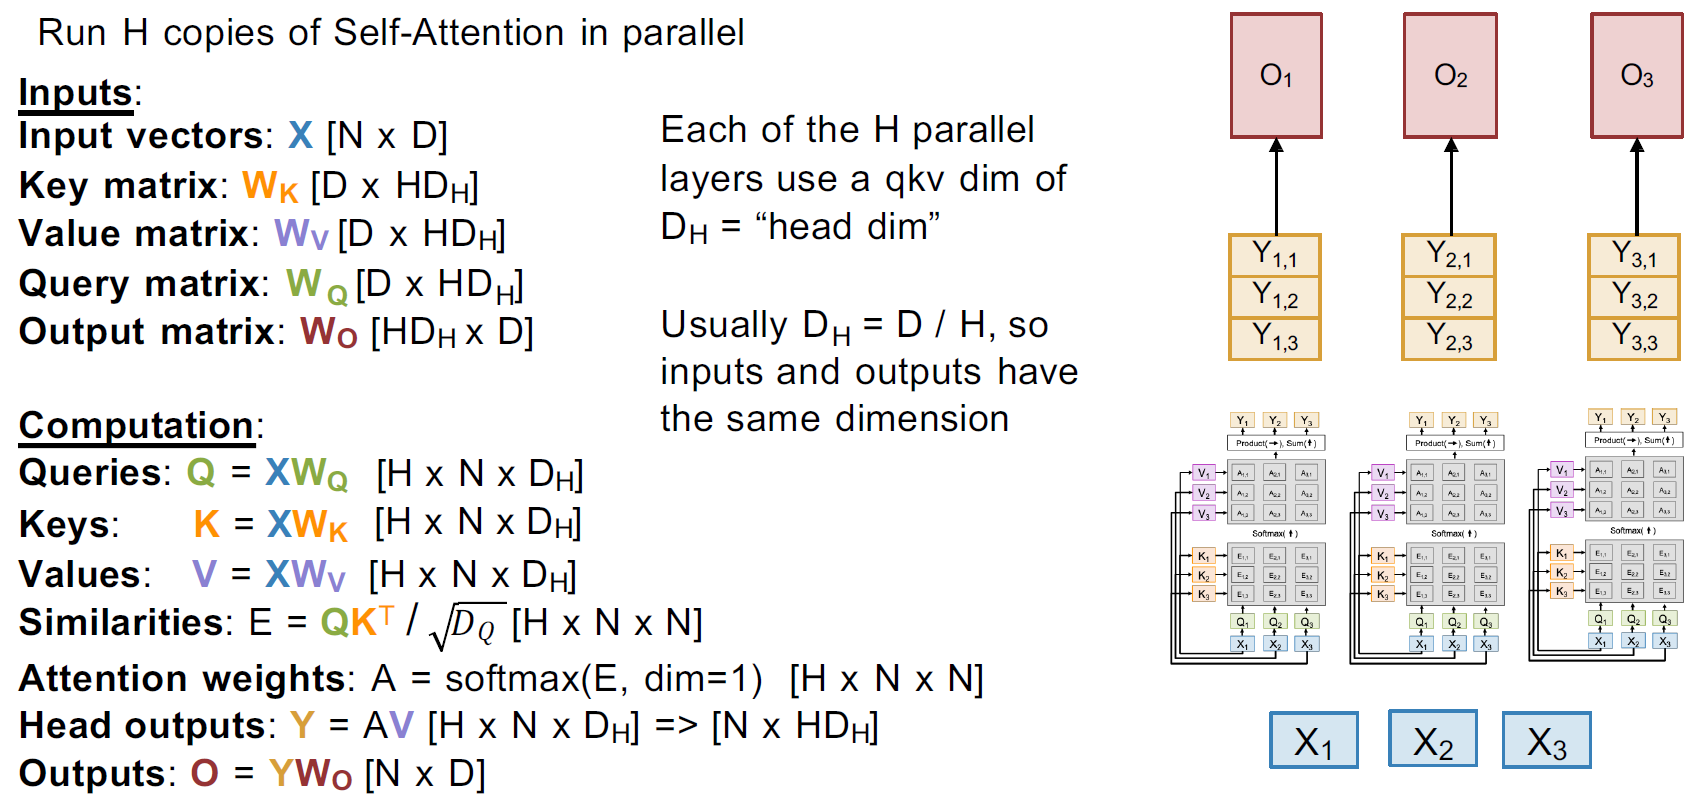
\includegraphics[width=\linewidth]{MultiHeadAttention.png}
    \caption{Multiheaded Self-Attention Layer}
\end{figure}

QKV projection - QK similarity - V weighting - output projection: compute $O(N^2)$, memory $O(N^2)$

flash attention - memory $O(N)$ (2+3 the same time)

\subsection*{Transformers}

\begin{figure}[H]
    \centering
    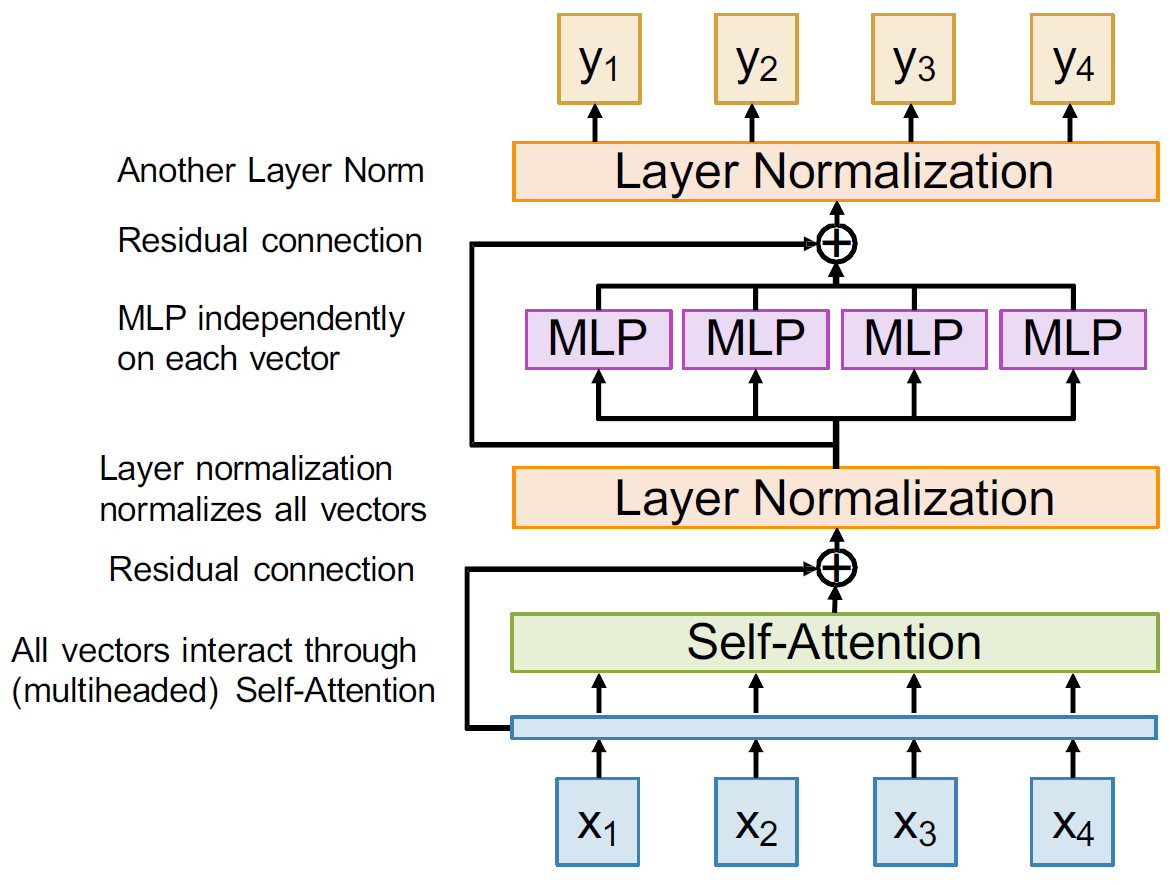
\includegraphics[width=0.6\linewidth]{TransformerBlock.png}
    \caption{Transformer Block}
\end{figure}

normalization per token, each submodule gets its own

$x \gets x+f(x)$ - keep activation in controlled range

Original(213M) - GPT-2(1.5B) - GPT-3(175B)

Pre-Norm: Move normalization inside residual

QK-Norm: Normalize keys and queries

SwiGLU: Different MLP architecture

Mixture of Experts (MoE): Learn E different MLPs, use A < E of them per token. Massively increase params, modest increase to compute cost.

\subsection*{Visual Transformers}

\entry{ViT}input - break into patches - flatten - transformer

low inductive bias, better on large data

\section{Generative Model}

\subsection*{Generative Models}

discriminative - learn $p(y|x)$ / generative - learn $p(x)$

conditional generative model: $p(x|y) = \frac{p(y|x)}{p(y)}p(x)$

model ambiguity - model $p(x|y)$ for many outputs

\begin{figure}[H]
    \centering
    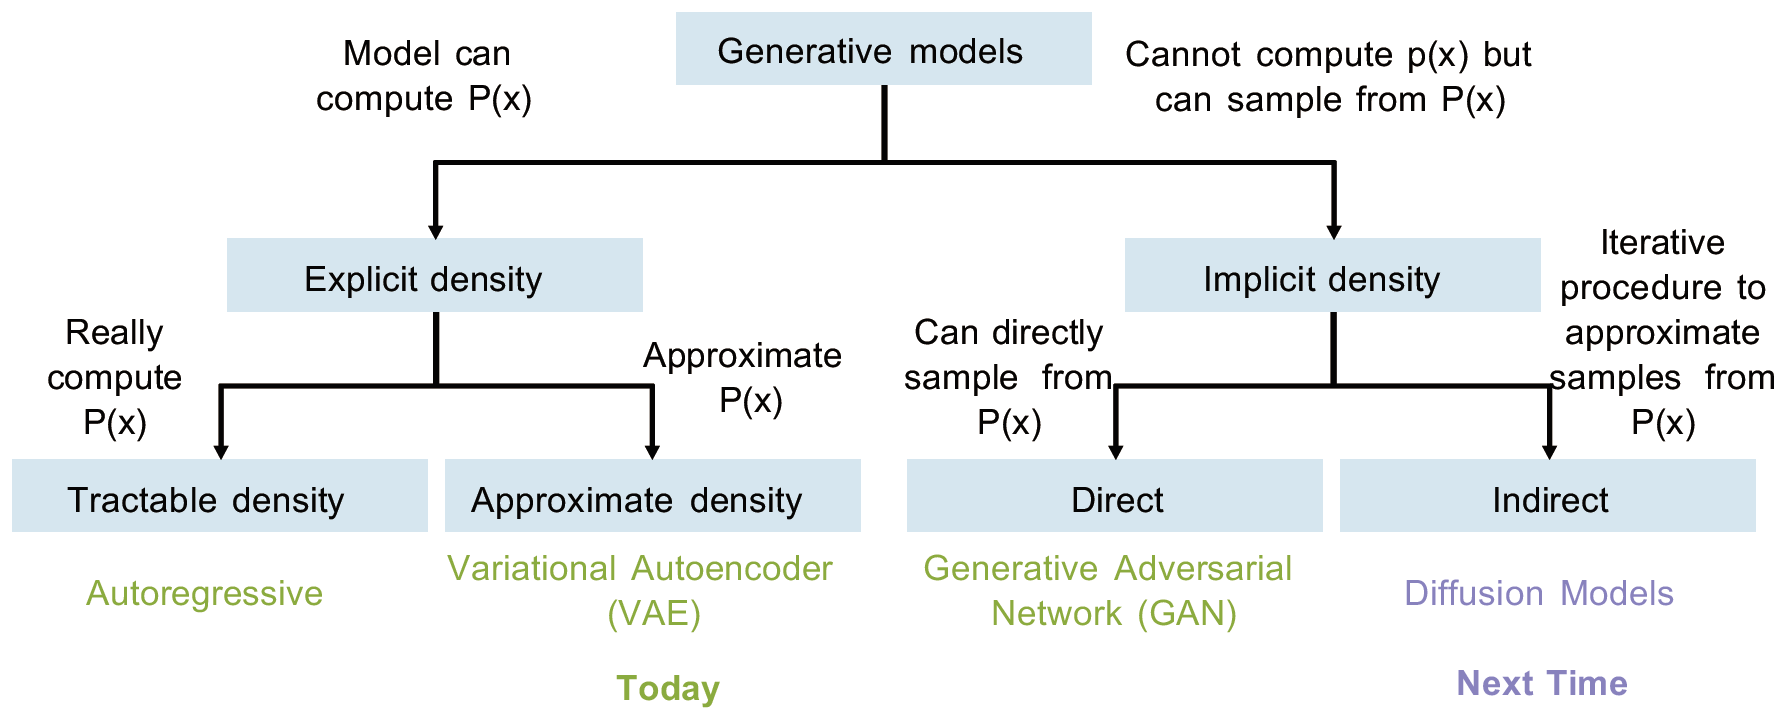
\includegraphics[width=\linewidth]{GenerativeModelTaxonomy.png}
    \caption{Taxonomy of Generative Models}
\end{figure}

\subsection*{Autoregressive Models}

$W^* = \arg\max_W\sum_i\log f(x^{(i)},W)$ loss function

for sequence $x$: $p(x) = \prod_{t=1}^T p(x_t|x_1,x_2,\cdots,x_{t-1})$

image as sequence of subpixels, use RNN/Transformer

too expensive - models as sequence of tiles

\subsection*{Variational Autoencoders (VAE)}

image x, z is latent factors used to generate x

\entry{Probalistic Autoencoder}$p_{\theta^*}(x|z^{(i)}), z^{(i)} \sim p_{\theta^*}(z)$

maximize $p_\theta(x) = \int p(z)p_\theta(x|z)dz$

intractable: Monte Carlo estimation (high variance)

$p(z)$: prior density; $p_\theta(z|x)$: posterior density

variational approximation: learn $q_\phi(z|x)$ (decoder)

\begin{figure}[H]
    \centering
    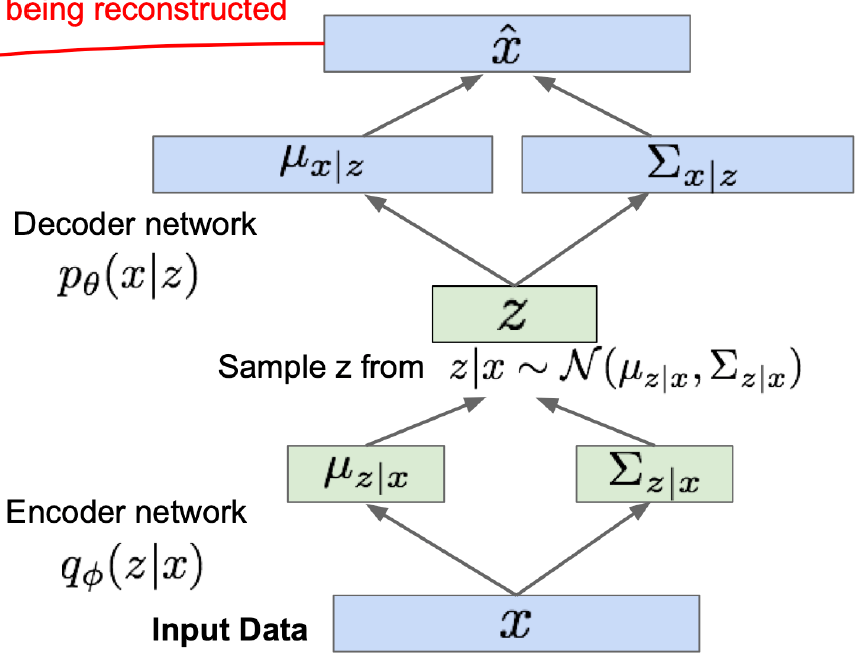
\includegraphics[width=0.6\linewidth]{VAE.png}
    \caption{Variational Autoencoder}
\end{figure}

\entry{loss}$\mathcal{L}=-\log p_{\theta,\phi}(x)$, maximize $\log p_\theta(x^{(i)}) = \mathbf{E}_z[\log p_\theta(x^{(i)}|z)] - D_{KL}(q_\phi(z|x^{(i)}) || p(z)) + D_{KL}(q_\phi(z|x^(i)) || p_\theta(z|x^{(i)}))$

$\mathcal{L}(x,\theta,\phi) = \mathbf{E}_z[\log p_\theta(x^{(i)}|z)] - D_{KL}(q_\phi(z|x^{(i)}) || p(z))$

in practice: $\Sigma_{z|x} = \mathbf{I}$

\begin{figure}[H]
    \centering
    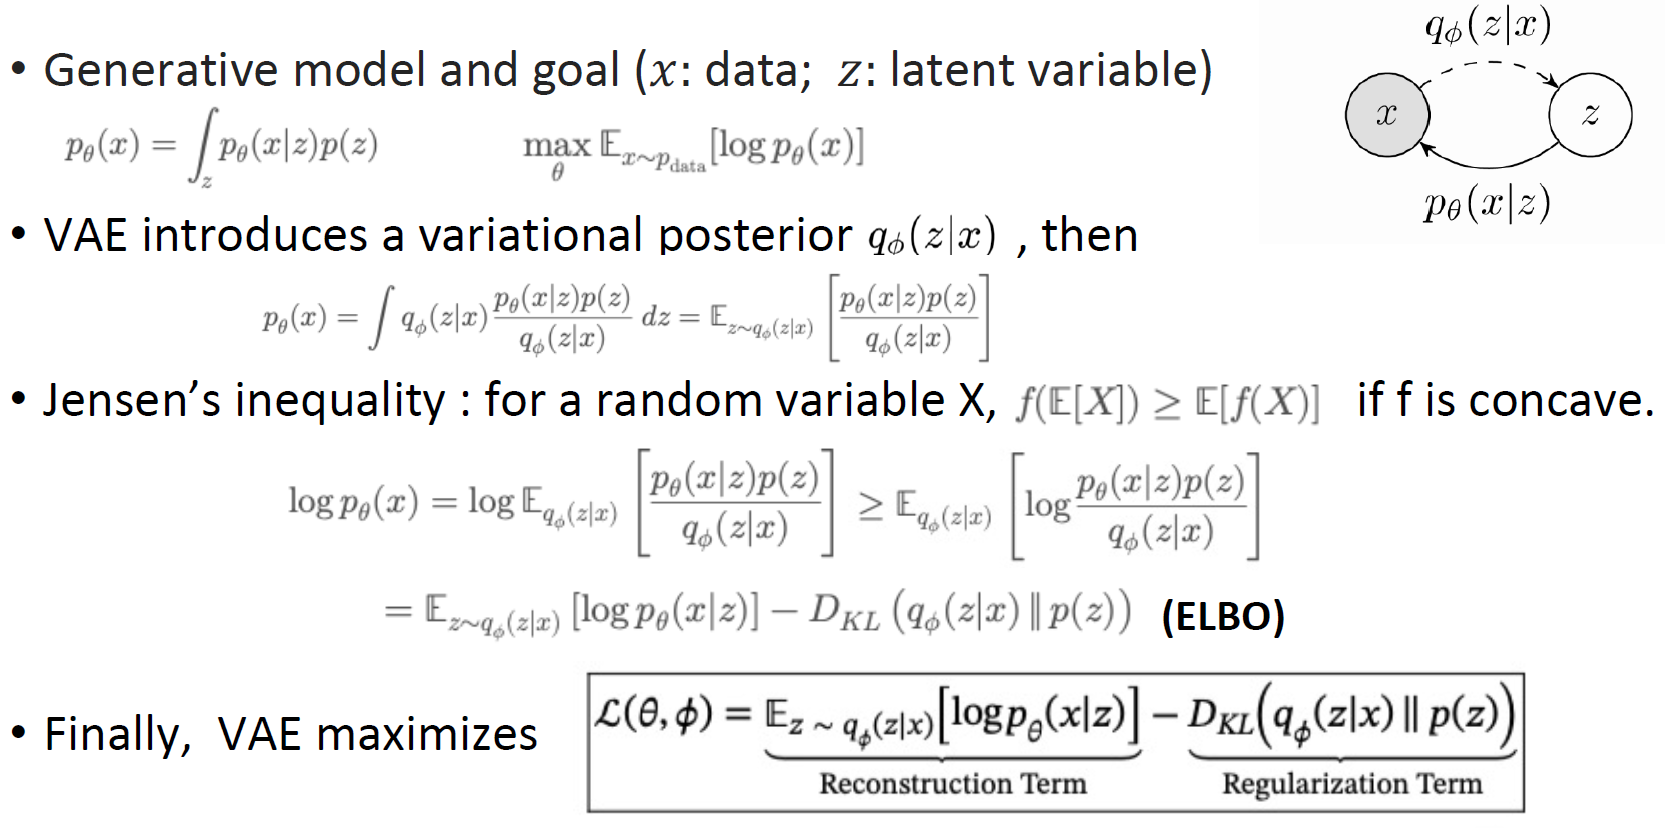
\includegraphics[width=\linewidth]{VAENutshell.png}
    \caption{VAE in a Nutshell}
\end{figure}

\subsection*{Generative Adversial Networks(GAN)}

not modeling any explicit density function

minimax obj func: $\min_{\theta_g} \max_{\theta_d} [E_{x\sim p_{data}} \log D_{\theta_d}(x) + E_{z\sim p_{(z)}} \log (1-D_{\theta_d} (G_{\theta_g}(z)))]$

discriminator($\theta_d$) max obj, generator($\theta_g$) min obj

generator-unsampling network with fractionally-strided convolutions; discriminator-convolutional network

Evaluation: nearest neighbors / user study / mode drop and mode collapse

$FID(r,g) = ||\mu_r - \mu_g||_2^2 +Tr(\Sigma_r + \Sigma_g -2(\Sigma_r\Sigma_g)^{1/2}$

lower FID - smaller distance between synthetic \& real

\subsection*{Diffusion Models}

limitations of VAE: single Gaussian latent code

hierarchical latent-variable model / Markov chain

forward process gradually adds Gaussian noise until data becomes nearly standard normal

reverse process learns to denoise step by step

\entry{Forward}$q(x_t|x_{t-1}) = \mathcal{N}(\sqrt{1-\beta_t}x_{t-1}, \beta_t I)$

let $\alpha_t = 1-\beta_t,\ \bar{\alpha}_t = \prod_{s=1}^t \alpha_s$

closed form: $x_t = \sqrt{\bar{\alpha}_t}x_0 + \sqrt{1-\bar{\alpha}_t}\epsilon,\ \epsilon\sim\mathcal{N}(0,I)$

\entry{Reverse denoising}learn $p_\theta(x_{t-1}|x_t)$

true reverse posterior is Gaussian; network predicts its mean or the noise

\entry{DDPM}training add known noise, then predict noise

$\mathcal{L}_{DDPM} = \mathbf{E}_{x_0,\epsilon,t} ||\epsilon-\epsilon_\theta(x_t,t)||_2^2$

sampling: start from $x_T \sim \mathcal{N}(0,I)$, iteratively denoise to $x_0$

can view diffusion as hierarchical VAE / score matching / solving an SDE

+: stable, high quality; -: many denoising steps, slow sampling

\subsection*{Latent Diffusion Models}

\entry{Why latent}pixel-space diffusion is expensive

compress image to latent $z \in \mathbb{R}^{H/D \times W/D \times C}$

$D=8,\ C=16$, so $256\times256\times3 \rightarrow 32\times32\times16$

\entry{LDM pipeline}VAE encoder/decoder + diffusion in latent space

train autoencoder, freeze encoder, add noise in latent space, denoise latent, decode to image

modern pipelines often use VAE + GAN + diffusion

VAE gives compression, GAN sharpens decoder output, diffusion models the latent distribution

\entry{Conditional diffusion}same denoising idea, but condition on text / image / control signal

most common: cross-attention with text embeddings

Stable Diffusion: pretrained text encoder + latent diffusion + decoder

\entry{Diffusion Transformer (DiT)}use standard transformer blocks as denoiser

inject timestep by scale / shift modulation; inject text or image by cross-attention / joint attention

\section{Large Models II}

\subsection*{Video Transformers}

video = image + time

\entry{Joint space-time attention}for $T$ frames and $N$ tokens per frame, full attention cost $O((TN)^2)$

captures all pairwise interactions but is expensive

\entry{Divided space-time attention}do temporal and spatial attention separately, cost $O(NT^2 + TN^2)$

main efficiency idea: factorize attention instead of attending jointly over all tokens

\entry{Video Swin Transformer}restrict attention to local windows, then shift windows

cheaper, good local motion modeling

\entry{MViT}multiscale vision transformer

reduce token count with pooling / hierarchy while increasing channel dimension

two broad strategies for efficient video: restrict attention range or reduce number of tokens

\subsection*{Foundation Models}

\entry{Families}

\begin{figure}[H]
    \centering
    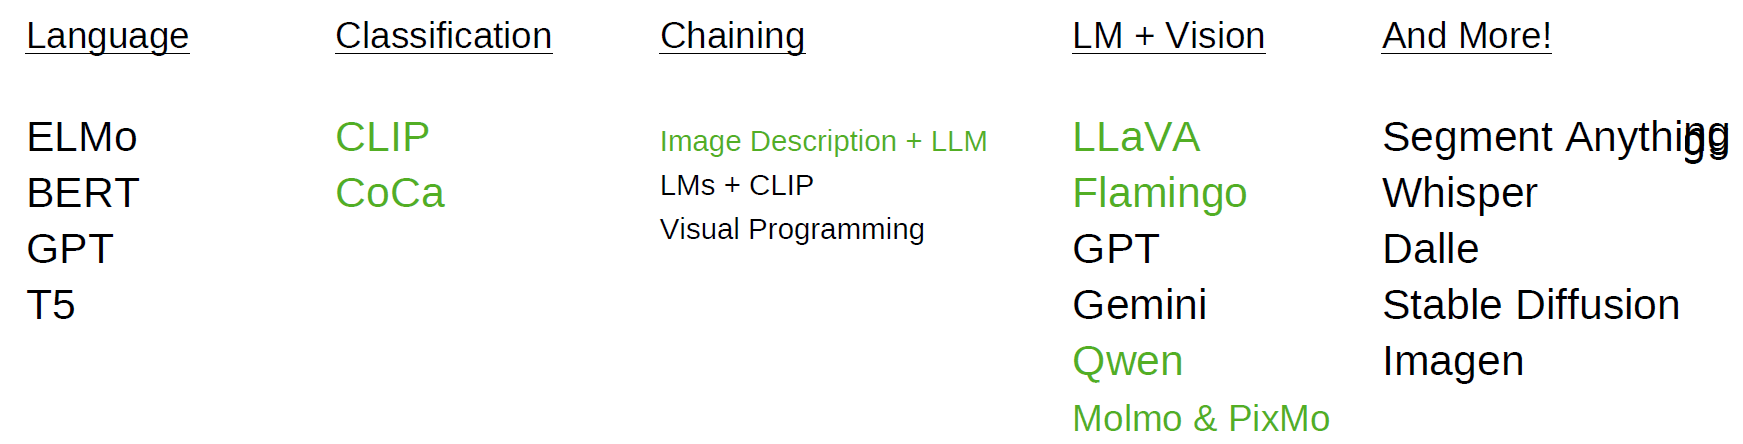
\includegraphics[width=0.8\linewidth]{FoundationModels.png}
    \caption{Foundation Models}
\end{figure}

\entry{CLIP}learn concepts without labels (self-supervised)

\entry{Contrastive learning}learn aligned image-text embedding space

image encoder+text encoder, similarity by dot product

$L_{i\rightarrow t} = -\frac{1}{B}\sum_i \log \frac{\exp(v_i^\top t_i/\tau)}{\sum_j \exp(v_i^\top t_j/\tau)}$

usually add the symmetric text$\rightarrow$image loss too

\entry{Usage}zero-shot classification by prompt engineering

create text vector for each category, compare image embedding with all prompt embeddings

linear probe on frozen CLIP features is also strong

CoCa: add a generative objective

+: open-vocabulary/reusable encoder/strong semantics

-: global image-text matching not enforce event struc

CLIP may know the right objects but still confuse who did what to whom

language compositionality and argument roles are weak

\entry{CLIP-Event}generate event-aware hard negatives / role-swapped negatives

helps distinguish same entities with different roles, but hard negatives alone can still teach shortcuts

\entry{Chain foundation models}

\entry{VidIL}Language Models with Image Descriptors are Strong Few-Shot Video-Language Learners

instead of training a full video-language model, chain frozen image-language models and a frozen LLM through text

\entry{Pipeline}sample frames $\rightarrow$ objects / events / attributes / frame captions / subtitle

$\rightarrow$ temporal-aware few-shot prompt $\rightarrow$ LLM output

\entry{Temporal prompts}use markers like First / Then / Finally (temporal order matters)

+: no video pretraining, few-shot capable, strong baseline for captioning / QA / event prediction

\entry{VS. Flamingo}compose existing models through language instead of training an integrated VLM

\entry{LLaVA}vision encoder(CLIP)+projector+autoregressive LLM

project visual features into language model token space, then decode text autoregressively

CLIP encode - strong visual semantics; penultimate-layer features are often better than final pooled output

\entry{Training recipe}first align visual features to the LLM, then do instruction tuning

inherits the autoregressive nature of LLMs, so naturally supports dialogue / description / QA

\entry{Flamingo}frozen vision encoder + frozen LM + newly inserted cross-attention layers

LM attends to visual tokens through cross-attention instead of collapsing everything into one vector

+: strong zero-shot / few-shot multimodal in-context learning

keeps more visual detail than pure CLIP-style global embeddings

LLaVA = projector into autoregressive LLM

Flamingo = frozen LM that reads visual tokens through cross-attention

\begin{figure}[H]
    \centering
    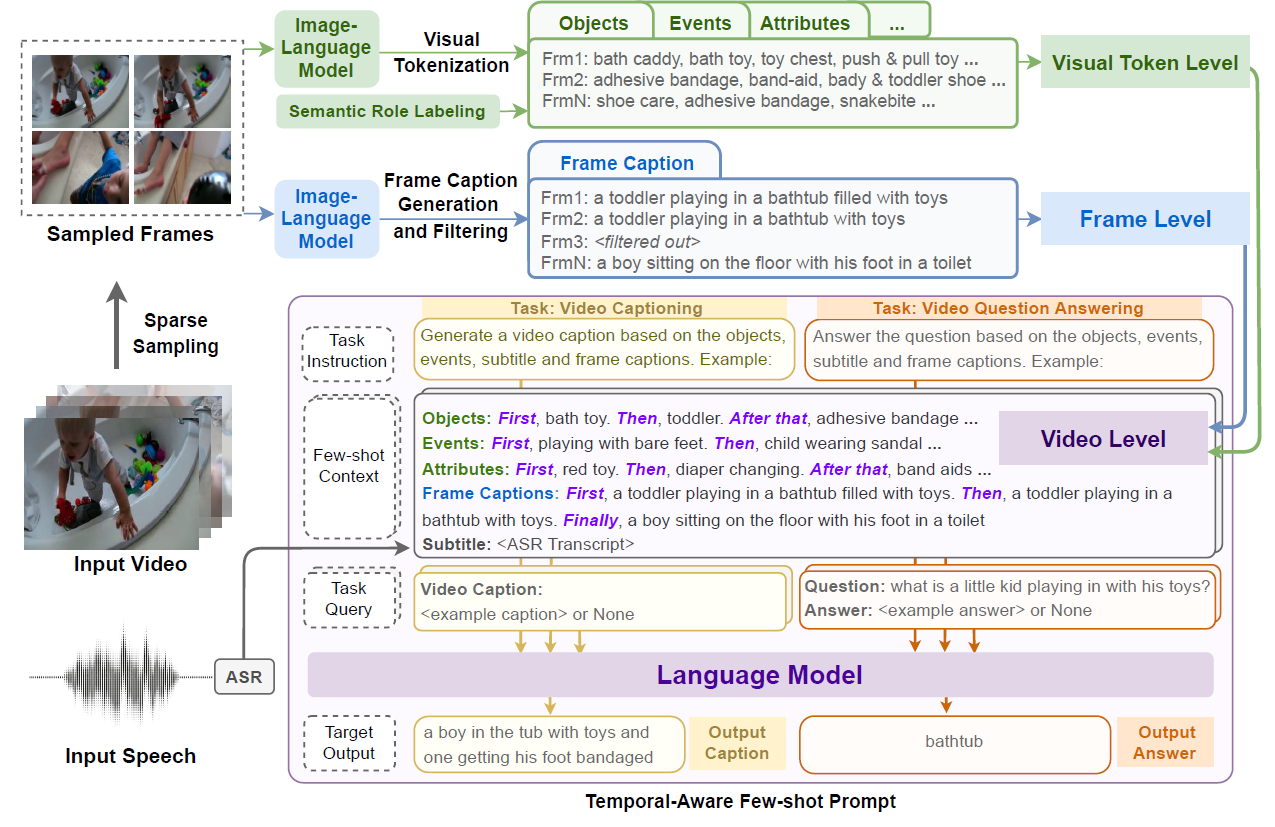
\includegraphics[width=\linewidth]{LargeModels.png}
    \caption{Large Models}
\end{figure}

% \section{Before Mid-term}

\end{multicols*}

\end{CJK*}
\end{document}
